% -------------------- Packages --------------------

\documentclass[lineno]{assignment}

% -------------------- Settings --------------------

% Title

\title{Homework of Chapter 2}
\author{Chen Xuyang}
\date{\today}
\institute{School of Mathematical Science}
\professor{Chen Xiongda}
\course{Operations Research}
\subject{Operations Research}
\keywords{}

% -------------------- New commands --------------------

\newcommand{\BR}{\symbb{R}}
\theoremstyle{plain}
\theoremheaderfont{\upshape\bfseries}
\theorembodyfont{\upshape}
\theoremsymbol{}
\newtheorem{lemma}{Lemma}

% -------------------- Document --------------------

\begin{document}
    \maketitle

    \begin{problem}
        Compute the gradient $\nabla f(x)$ and Hessian $\nabla^{2}f(x)$ of the Rosenbrock function
        \begin{equation}
            f(x)=100(x_{2}-x_{1}^{2})^{2}+(1-x_{1})^{2}.
        \end{equation}
        Show that $x^{*}=(1,1)^{T}$ is the only local minimizer of this function, and that the Hessian matrix at that point is positive definite.
    \end{problem}
    \begin{solution}
        Calculate the gradient and Hessian of $f$, we have
        \begin{equation}
            \nabla f =
            \begin{bmatrix}
                400x_1^3+2x_1-400x_1x_2-2\\
                -200x_1^2+200x_2
            \end{bmatrix},
        \end{equation}
        and
        \begin{equation}
            \nabla^{2}f(x) =
            \begin{bmatrix}
                1200x_1^2-400x_2+2 & -400x_1\\
                -400x_1 & 200
            \end{bmatrix}.
        \end{equation}
        It's obvious that $\nabla f(x)=0$ if and only if $x=(1,1)^{T}$, and
        \begin{equation}
            \nabla^{2}f(1, 1) =
            \begin{bmatrix}
                802 & -400\\
                -400 & 200
            \end{bmatrix}
        \end{equation}
        is positive definite by testing Sylvester's criterion.
    \end{solution}
    \begin{problem}
        Show that the function $f(x)=8x_1+12x_2+x_1^2-2x_2^2$ has only one stationary point, and that it is neither a maximum or minimum, but a saddle point. Sketch the contour lines of $f$.
    \end{problem}
    \begin{solution}
        Calculate the gradient of $f$
        \begin{equation}
            \nabla f =
            \begin{bmatrix}
                2x_1+8\\
                -4x_2+12
            \end{bmatrix}.
        \end{equation}
        Then we can find out $f$ has only one stationary point, that is $(-4, 3)^T$. At that point, the Hessian
        \begin{equation}
            \nabla^{2}f =
            \begin{bmatrix}
                2 & 0\\
                0 & -4
            \end{bmatrix}
        \end{equation}
        is indefinite. Hence it is a saddle point.
        \begin{figure}[H]
            \centering
            % This file was created by matlab2tikz.
%
%The latest updates can be retrieved from
%  http://www.mathworks.com/matlabcentral/fileexchange/22022-matlab2tikz-matlab2tikz
%where you can also make suggestions and rate matlab2tikz.
%
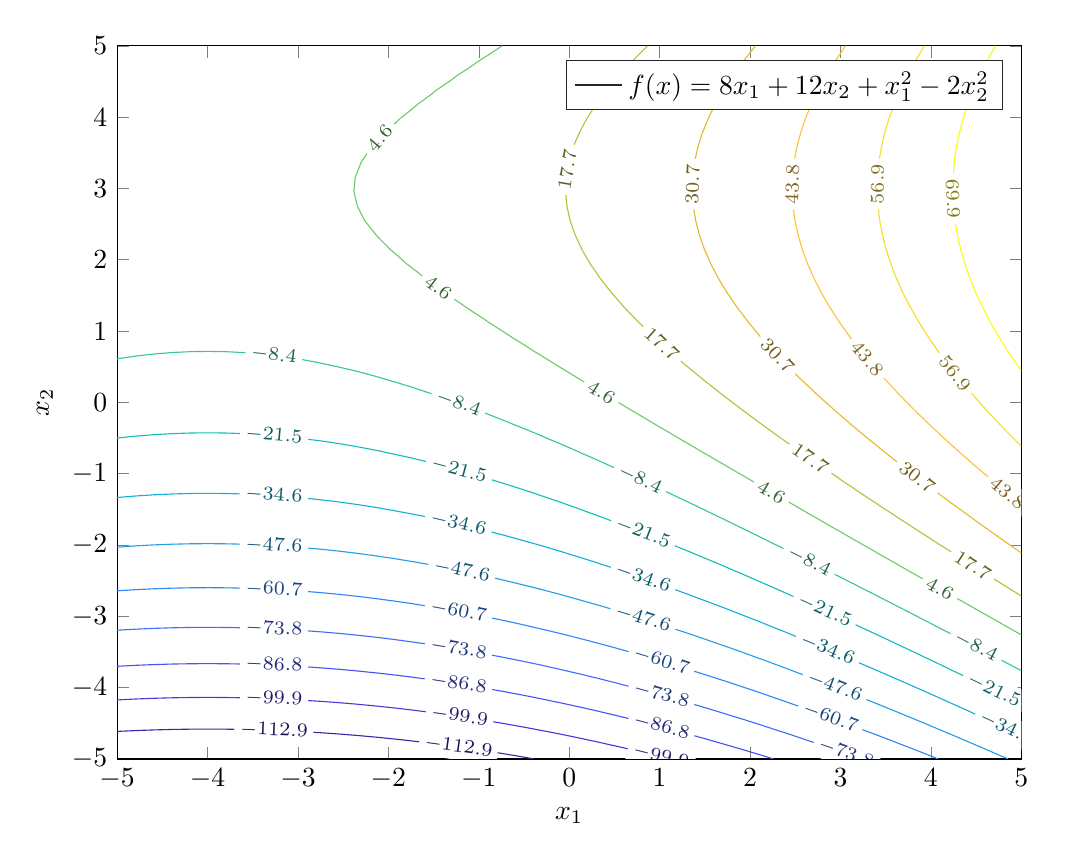
\begin{tikzpicture}

\begin{axis}[%
width=4.521in,
height=3.566in,
at={(0.758in,0.481in)},
xlabel={$x_1$},
ylabel={$x_2$},
scale only axis,
colormap={mymap}{[1pt] rgb(0pt)=(0.2422,0.1504,0.6603); rgb(1pt)=(0.25039,0.164995,0.707614); rgb(2pt)=(0.257771,0.181781,0.751138); rgb(3pt)=(0.264729,0.197757,0.795214); rgb(4pt)=(0.270648,0.214676,0.836371); rgb(5pt)=(0.275114,0.234238,0.870986); rgb(6pt)=(0.2783,0.255871,0.899071); rgb(7pt)=(0.280333,0.278233,0.9221); rgb(8pt)=(0.281338,0.300595,0.941376); rgb(9pt)=(0.281014,0.322757,0.957886); rgb(10pt)=(0.279467,0.344671,0.971676); rgb(11pt)=(0.275971,0.366681,0.982905); rgb(12pt)=(0.269914,0.3892,0.9906); rgb(13pt)=(0.260243,0.412329,0.995157); rgb(14pt)=(0.244033,0.435833,0.998833); rgb(15pt)=(0.220643,0.460257,0.997286); rgb(16pt)=(0.196333,0.484719,0.989152); rgb(17pt)=(0.183405,0.507371,0.979795); rgb(18pt)=(0.178643,0.528857,0.968157); rgb(19pt)=(0.176438,0.549905,0.952019); rgb(20pt)=(0.168743,0.570262,0.935871); rgb(21pt)=(0.154,0.5902,0.9218); rgb(22pt)=(0.146029,0.609119,0.907857); rgb(23pt)=(0.138024,0.627629,0.89729); rgb(24pt)=(0.124814,0.645929,0.888343); rgb(25pt)=(0.111252,0.6635,0.876314); rgb(26pt)=(0.0952095,0.679829,0.859781); rgb(27pt)=(0.0688714,0.694771,0.839357); rgb(28pt)=(0.0296667,0.708167,0.816333); rgb(29pt)=(0.00357143,0.720267,0.7917); rgb(30pt)=(0.00665714,0.731214,0.766014); rgb(31pt)=(0.0433286,0.741095,0.73941); rgb(32pt)=(0.0963952,0.75,0.712038); rgb(33pt)=(0.140771,0.7584,0.684157); rgb(34pt)=(0.1717,0.766962,0.655443); rgb(35pt)=(0.193767,0.775767,0.6251); rgb(36pt)=(0.216086,0.7843,0.5923); rgb(37pt)=(0.246957,0.791795,0.556743); rgb(38pt)=(0.290614,0.79729,0.518829); rgb(39pt)=(0.340643,0.8008,0.478857); rgb(40pt)=(0.3909,0.802871,0.435448); rgb(41pt)=(0.445629,0.802419,0.390919); rgb(42pt)=(0.5044,0.7993,0.348); rgb(43pt)=(0.561562,0.794233,0.304481); rgb(44pt)=(0.617395,0.787619,0.261238); rgb(45pt)=(0.671986,0.779271,0.2227); rgb(46pt)=(0.7242,0.769843,0.191029); rgb(47pt)=(0.773833,0.759805,0.16461); rgb(48pt)=(0.820314,0.749814,0.153529); rgb(49pt)=(0.863433,0.7406,0.159633); rgb(50pt)=(0.903543,0.733029,0.177414); rgb(51pt)=(0.939257,0.728786,0.209957); rgb(52pt)=(0.972757,0.729771,0.239443); rgb(53pt)=(0.995648,0.743371,0.237148); rgb(54pt)=(0.996986,0.765857,0.219943); rgb(55pt)=(0.995205,0.789252,0.202762); rgb(56pt)=(0.9892,0.813567,0.188533); rgb(57pt)=(0.978629,0.838629,0.176557); rgb(58pt)=(0.967648,0.8639,0.16429); rgb(59pt)=(0.96101,0.889019,0.153676); rgb(60pt)=(0.959671,0.913457,0.142257); rgb(61pt)=(0.962795,0.937338,0.12651); rgb(62pt)=(0.969114,0.960629,0.106362); rgb(63pt)=(0.9769,0.9839,0.0805)},
xmin=-5,
xmax=5,
ymin=-5,
ymax=5,
axis background/.style={fill=white},
legend style={legend cell align=left, align=left, draw=white!15!black}
]
\addplot[contour prepared, contour prepared format=matlab] table[row sep=crcr] {%
%
-112.937317784257	27\\
-5	-4.61345612515563\\
-4.79591836734694	-4.60154685216262\\
-4.59183673469388	-4.59234423212256\\
-4.57589285714287	-4.59183673469388\\
-4.38775510204082	-4.58568509147528\\
-4.18367346938776	-4.58179252627481\\
-3.97959183673469	-4.58068036478897\\
-3.77551020408163	-4.58234860701774\\
-3.57142857142857	-4.58679725296113\\
-3.42916012558869	-4.59183673469388\\
-3.36734693877551	-4.59396822389433\\
-3.16326530612245	-4.60371217452498\\
-2.95918367346939	-4.61616277810859\\
-2.75510204081633	-4.63132003464516\\
-2.55102040816327	-4.64918394413468\\
-2.3469387755102	-4.66975450657717\\
-2.14285714285714	-4.69303172197261\\
-1.93877551020408	-4.71901559032101\\
-1.73469387755102	-4.74770611162237\\
-1.53061224489796	-4.77910328587669\\
-1.42998866213152	-4.79591836734694\\
-1.3265306122449	-4.81276037546802\\
-1.12244897959184	-4.84861968043031\\
-0.918367346938775	-4.88711569899278\\
-0.714285714285714	-4.92824843115541\\
-0.510204081632653	-4.97201787691821\\
-0.38714633580705	-5\\
-99.875052061641	35\\
-5	-4.17183732282538\\
-4.79591836734694	-4.15889842968888\\
-4.59183673469388	-4.1489001940834\\
-4.38775510204082	-4.14184261600894\\
-4.18367346938776	-4.13772569546551\\
-3.97959183673469	-4.1365494324531\\
-3.77551020408163	-4.13831382697171\\
-3.57142857142857	-4.14301887902135\\
-3.36734693877551	-4.15066458860201\\
-3.16326530612245	-4.1612509557137\\
-2.95918367346939	-4.17477798035641\\
-2.84894314868805	-4.18367346938776\\
-2.75510204081633	-4.19103355627965\\
-2.55102040816327	-4.20989824501229\\
-2.3469387755102	-4.23162121991654\\
-2.14285714285714	-4.2562024809924\\
-1.93877551020408	-4.28364202823987\\
-1.73469387755102	-4.31393986165895\\
-1.53061224489796	-4.34709598124964\\
-1.3265306122449	-4.38311038701195\\
-1.30214585834334	-4.38775510204082\\
-1.12244897959184	-4.42105043652338\\
-0.918367346938775	-4.46164433075683\\
-0.714285714285714	-4.50501862870489\\
-0.510204081632653	-4.55117333036757\\
-0.340619202226344	-4.59183673469388\\
-0.306122448979592	-4.59988902722893\\
-0.102040816326531	-4.65023277215395\\
0.102040816326531	-4.70328317003194\\
0.306122448979592	-4.75904022086288\\
0.434854497354498	-4.79591836734694\\
0.510204081632653	-4.81694615830828\\
0.714285714285714	-4.8765358856721\\
0.918367346938775	-4.93876232663608\\
1.11104197776672	-5\\
-86.8127863390254	43\\
-5	-3.70050084253885\\
-4.79591836734694	-3.68677057979155\\
-4.59183673469388	-3.676160831305\\
-4.38775510204082	-3.6686715970792\\
-4.18367346938776	-3.66430287711415\\
-3.97959183673469	-3.66305467140985\\
-3.77551020408163	-3.6649269799663\\
-3.57142857142857	-3.6699198027835\\
-3.36734693877551	-3.67803313986145\\
-3.16326530612245	-3.68926699120015\\
-2.95918367346939	-3.7036213567996\\
-2.75510204081633	-3.7210962366598\\
-2.55102040816327	-3.74169163078075\\
-2.3469387755102	-3.76540753916245\\
-2.27011153298529	-3.77551020408163\\
-2.14285714285714	-3.79174741113063\\
-1.93877551020408	-3.82081541815539\\
-1.73469387755102	-3.85291134257858\\
-1.53061224489796	-3.88803518440017\\
-1.3265306122449	-3.92618694362018\\
-1.12244897959184	-3.9673666202386\\
-1.06601202124686	-3.97959183673469\\
-0.918367346938775	-4.01065253190613\\
-0.714285714285714	-4.05652678939011\\
-0.510204081632653	-4.10534170440511\\
-0.306122448979592	-4.15709727695113\\
-0.206961816984861	-4.18367346938776\\
-0.102040816326531	-4.21100583090379\\
0.102040816326531	-4.26702823986738\\
0.306122448979592	-4.32590893500257\\
0.510204081632653	-4.38764791630938\\
0.510542712660283	-4.38775510204082\\
0.714285714285714	-4.45048796085192\\
0.918367346938775	-4.51610548851693\\
1.12244897959184	-4.58450341989657\\
1.14347496811224	-4.59183673469388\\
1.3265306122449	-4.65398825312618\\
1.53061224489796	-4.72598522167488\\
1.72166149068323	-4.79591836734694\\
1.73469387755102	-4.80056557506724\\
1.93877551020408	-4.87597558403206\\
2.14285714285714	-4.95402230659706\\
2.25915366146458	-5\\
-73.7505206164098	52\\
-5	-3.1943428837333\\
-4.79591836734694	-3.17971814132819\\
-4.59183673469388	-3.16841720401516\\
-4.46003401360545	-3.16326530612245\\
-4.38775510204082	-3.16034494605923\\
-4.18367346938776	-3.15553494124923\\
-3.97959183673469	-3.15416065416065\\
-3.77551020408163	-3.15622208479351\\
-3.57142857142857	-3.1617192331478\\
-3.53610675039246	-3.16326530612245\\
-3.36734693877551	-3.1704114870704\\
-3.16326530612245	-3.18237718540185\\
-2.95918367346939	-3.19766668882537\\
-2.75510204081633	-3.21627999734096\\
-2.55102040816327	-3.23821711094861\\
-2.3469387755102	-3.26347802964834\\
-2.14285714285714	-3.29206275344014\\
-1.93877551020408	-3.323971282324\\
-1.73469387755102	-3.35920361629994\\
-1.69159042927516	-3.36734693877551\\
-1.53061224489796	-3.39680036052276\\
-1.3265306122449	-3.43735917079766\\
-1.12244897959184	-3.48113693426898\\
-0.918367346938775	-3.52813365093672\\
-0.742412349555207	-3.57142857142857\\
-0.714285714285714	-3.57813767708918\\
-0.510204081632653	-3.62993821381764\\
-0.306122448979592	-3.68485926480684\\
-0.102040816326531	-3.74290083005679\\
0.00676801332778076	-3.77551020408163\\
0.102040816326531	-3.80321564827711\\
0.306122448979592	-3.86559074668443\\
0.510204081632653	-3.93099376249016\\
0.655138161459274	-3.97959183673469\\
0.714285714285714	-3.9988531435629\\
0.918367346938775	-4.06825266129507\\
1.12244897959184	-4.14059283655825\\
1.23923788265306	-4.18367346938776\\
1.3265306122449	-4.2149717029669\\
1.53061224489796	-4.29100211513177\\
1.73469387755102	-4.36989081346824\\
1.77929213643499	-4.38775510204082\\
1.93877551020408	-4.44989712506256\\
2.14285714285714	-4.53219707501529\\
2.2859143657463	-4.59183673469388\\
2.3469387755102	-4.61660260921345\\
2.55102040816327	-4.70213284252693\\
2.75510204081633	-4.79036972879337\\
2.76755344995141	-4.79591836734694\\
2.95918367346939	-4.87910668143226\\
3.16326530612245	-4.9703369719981\\
3.22775739509287	-5\\
-60.6882548937943	57\\
-5	-2.64214801444043\\
-4.79591836734694	-2.62593936491564\\
-4.59183673469388	-2.61341449937376\\
-4.38775510204082	-2.60457341781478\\
-4.18367346938776	-2.59941612023871\\
-3.97959183673469	-2.59794260664555\\
-3.77551020408163	-2.60015287703529\\
-3.57142857142857	-2.60604693140794\\
-3.36734693877551	-2.6156247697635\\
-3.16326530612245	-2.62888639210197\\
-2.95918367346939	-2.64583179842334\\
-2.75510204081633	-2.66646098872762\\
-2.55102040816327	-2.69077396301481\\
-2.3469387755102	-2.7187707212849\\
-2.14285714285714	-2.75045126353791\\
-2.11601828231293	-2.75510204081633\\
-1.93877551020408	-2.78474543127356\\
-1.73469387755102	-2.82243298016071\\
-1.53061224489796	-2.86367595818815\\
-1.3265306122449	-2.9084743653559\\
-1.12244897959184	-2.95682820166394\\
-1.11318842605536	-2.95918367346939\\
-0.918367346938775	-3.00706898921185\\
-0.714285714285714	-3.06066618566619\\
-0.510204081632653	-3.11769909984196\\
-0.356418135435994	-3.16326530612245\\
-0.306122448979592	-3.1776823107093\\
-0.102040816326531	-3.23950508542179\\
0.102040816326531	-3.30465166522635\\
0.288909253021595	-3.36734693877551\\
0.306122448979592	-3.37293986995429\\
0.510204081632653	-3.44246925899697\\
0.714285714285714	-3.51521760123608\\
0.865293151158767	-3.57142857142857\\
0.918367346938775	-3.59058072770393\\
1.12244897959184	-3.66734537851838\\
1.3265306122449	-3.74723054359358\\
1.39606030382078	-3.77551020408163\\
1.53061224489796	-3.82861230545631\\
1.73469387755102	-3.91218282565252\\
1.89355287569573	-3.97959183673469\\
1.93877551020408	-3.99822825383756\\
2.14285714285714	-4.08527171675587\\
2.3469387755102	-4.1752558372052\\
2.36542560061999	-4.18367346938776\\
2.55102040816327	-4.26581346824444\\
2.75510204081633	-4.35899359743898\\
2.81622023809524	-4.38775510204082\\
2.95918367346939	-4.45319885447367\\
3.16326530612245	-4.5494008229995\\
3.25075957349232	-4.59183673469388\\
3.36734693877551	-4.64688328912467\\
3.57142857142857	-4.74594678720295\\
3.67163753799392	-4.79591836734694\\
3.77551020408163	-4.84637847387017\\
3.97959183673469	-4.94815561883668\\
4.08092403628118	-5\\
-47.6259891711787	64\\
-5	-2.03017846814839\\
-4.79591836734694	-2.012001156738\\
-4.59183673469388	-1.99795505246633\\
-4.38775510204082	-1.98804015533339\\
-4.18367346938776	-1.98225646533917\\
-3.97959183673469	-1.98060398248368\\
-3.77551020408163	-1.98308270676692\\
-3.57142857142857	-1.98969263818888\\
-3.36734693877551	-2.00043377674957\\
-3.16326530612245	-2.01530612244898\\
-2.95918367346939	-2.03430967528712\\
-2.75510204081633	-2.05744443526398\\
-2.55102040816327	-2.08471040237958\\
-2.3469387755102	-2.11610757663389\\
-2.19328429046037	-2.14285714285714\\
-2.14285714285714	-2.15129436988803\\
-1.93877551020408	-2.18941078376876\\
-1.73469387755102	-2.23149765742873\\
-1.53061224489796	-2.27755499086794\\
-1.3265306122449	-2.3275827840864\\
-1.25337635054022	-2.3469387755102\\
-1.12244897959184	-2.3802835741038\\
-0.918367346938775	-2.43608117404265\\
-0.714285714285714	-2.49570052740197\\
-0.536328989427099	-2.55102040816327\\
-0.510204081632653	-2.55884844912694\\
-0.306122448979592	-2.62368304722611\\
-0.102040816326531	-2.69220142930819\\
0.0757496876301529	-2.75510204081633\\
0.102040816326531	-2.76407949939558\\
0.306122448979592	-2.8373213396857\\
0.510204081632653	-2.91411860911612\\
0.624661368972366	-2.95918367346939\\
0.714285714285714	-2.9932831718546\\
0.918367346938775	-3.0743661100804\\
1.12244897959184	-3.15888476602762\\
1.13261320153061	-3.16326530612245\\
1.3265306122449	-3.24411686498704\\
1.53061224489796	-3.33253008043608\\
1.60806713989944	-3.36734693877551\\
1.73469387755102	-3.42247151226421\\
1.93877551020408	-3.51453357368184\\
2.06063844456701	-3.57142857142857\\
2.14285714285714	-3.60864070398802\\
2.3469387755102	-3.70412844036697\\
2.49467191940067	-3.77551020408163\\
2.55102040816327	-3.80192878338279\\
2.75510204081633	-3.90063889057107\\
2.91347789115646	-3.97959183673469\\
2.95918367346939	-4.00172028465565\\
3.16326530612245	-4.10346703522908\\
3.3196227929374	-4.18367346938776\\
3.36734693877551	-4.20746870176642\\
3.57142857142857	-4.3120819756474\\
3.71512700825011	-4.38775510204082\\
3.77551020408163	-4.41868709336596\\
3.97959183673469	-4.52601067675026\\
4.10160276231705	-4.59183673469388\\
4.18367346938776	-4.63494018296974\\
4.38775510204082	-4.74483029285985\\
4.48035223704867	-4.79591836734694\\
4.59183673469388	-4.85583768391077\\
4.79591836734694	-4.96816168327796\\
4.85243868189478	-5\\
-34.5637234485631	68\\
-5	-1.33364290416628\\
-4.9298469387755	-1.3265306122449\\
-4.79591836734694	-1.31229665779355\\
-4.59183673469388	-1.29553633047422\\
-4.38775510204082	-1.28370551118998\\
-4.18367346938776	-1.27680419994085\\
-3.97959183673469	-1.27483239672681\\
-3.77551020408163	-1.27779010154787\\
-3.57142857142857	-1.28567731440402\\
-3.36734693877551	-1.29849403529528\\
-3.16326530612245	-1.31624026422163\\
-3.07065217391305	-1.3265306122449\\
-2.95918367346939	-1.33834524593247\\
-2.75510204081633	-1.36467835982319\\
-2.55102040816327	-1.39571381548011\\
-2.3469387755102	-1.43145161290323\\
-2.14285714285714	-1.47189175209254\\
-1.93877551020408	-1.51703423304806\\
-1.88318251829034	-1.53061224489796\\
-1.73469387755102	-1.56528139890317\\
-1.53061224489796	-1.61742560460308\\
-1.3265306122449	-1.67406500044952\\
-1.12413715486195	-1.73469387755102\\
-1.12244897959184	-1.7351782485146\\
-0.918367346938775	-1.79803883578748\\
-0.714285714285714	-1.86520494273659\\
-0.510204081632653	-1.93667656936192\\
-0.504551252319111	-1.93877551020408\\
-0.306122448979592	-2.00947079236553\\
-0.102040816326531	-2.08631124514583\\
0.0404779258642218	-2.14285714285714\\
0.102040816326531	-2.16633248630191\\
0.306122448979592	-2.24812395775431\\
0.510204081632653	-2.33388588898595\\
0.539890735055083	-2.3469387755102\\
0.714285714285714	-2.42074638844302\\
0.918367346938775	-2.51093976916609\\
1.00537166085946	-2.55102040816327\\
1.12244897959184	-2.60300780962204\\
1.3265306122449	-2.69731267958447\\
1.44688890593831	-2.75510204081633\\
1.53061224489796	-2.79390066130982\\
1.73469387755102	-2.89203050558202\\
1.86946981589839	-2.95918367346939\\
1.93877551020408	-2.9925530818388\\
2.14285714285714	-3.09425032639318\\
2.27682739762572	-3.16326530612245\\
2.3469387755102	-3.19820680715283\\
2.55102040816327	-3.30323904806222\\
2.67176349067234	-3.36734693877551\\
2.75510204081633	-3.41019925320286\\
2.95918367346939	-3.51835608060259\\
3.05643211041642	-3.57142857142857\\
3.16326530612245	-3.62794888597641\\
3.36734693877551	-3.73903919365912\\
3.43251644920263	-3.77551020408163\\
3.57142857142857	-3.85094319626961\\
3.77551020408163	-3.96479289044995\\
3.80135085122132	-3.97959183673469\\
3.97959183673469	-4.07872875374934\\
4.1635101010101	-4.18367346938776\\
4.18367346938776	-4.19485651403419\\
4.38775510204082	-4.31090293260161\\
4.51966002747253	-4.38775510204082\\
4.59183673469388	-4.42866179169215\\
4.79591836734694	-4.54710698993494\\
4.87122027710167	-4.59183673469388\\
5	-4.66630352406214\\
-21.5014577259475	69\\
-5	-0.499816693144325\\
-4.79591836734694	-0.472931687645119\\
-4.59183673469388	-0.45215691066846\\
-4.38775510204082	-0.437492362214347\\
-4.18367346938776	-0.428938042282782\\
-3.97959183673469	-0.426493950873763\\
-3.77551020408163	-0.430160087987291\\
-3.57142857142857	-0.439936453623367\\
-3.36734693877551	-0.455823047781988\\
-3.16326530612245	-0.477819870463156\\
-2.95918367346939	-0.505926921666871\\
-2.93367346938776	-0.510204081632653\\
-2.75510204081633	-0.538452669203275\\
-2.55102040816327	-0.576501787155541\\
-2.3469387755102	-0.620315922979362\\
-2.14285714285714	-0.669895076674739\\
-1.97916666666667	-0.714285714285714\\
-1.93877551020408	-0.724653497762742\\
-1.73469387755102	-0.782494816108262\\
-1.53061224489796	-0.845792862599586\\
-1.3265306122449	-0.914547637236714\\
-1.31602641056423	-0.918367346938775\\
-1.12244897959184	-0.985185952553611\\
-0.918367346938775	-1.06081011084637\\
-0.762689691261122	-1.12244897959184\\
-0.714285714285714	-1.1406881593217\\
-0.510204081632653	-1.22251799270433\\
-0.306122448979592	-1.30927733412206\\
-0.267719991222297	-1.3265306122449\\
-0.102040816326531	-1.39753597291451\\
0.102040816326531	-1.48970187153202\\
0.188230632058648	-1.53061224489796\\
0.306122448979592	-1.58410500764182\\
0.510204081632653	-1.68120111480716\\
0.617662994401299	-1.73469387755102\\
0.714285714285714	-1.78076293808663\\
0.918367346938775	-1.88237320244554\\
1.02704496432719	-1.93877551020408\\
1.12244897959184	-1.98628439229943\\
1.3265306122449	-2.09204329505081\\
1.42089918674237	-2.14285714285714\\
1.53061224489796	-2.19963471770031\\
1.73469387755102	-2.3092194076074\\
1.80248323105466	-2.3469387755102\\
1.93877551020408	-2.41993426584117\\
2.14285714285714	-2.53305816708706\\
2.17420301453915	-2.55102040816327\\
2.3469387755102	-2.64643041332056\\
2.53745802118316	-2.75510204081633\\
2.55102040816327	-2.76256844201095\\
2.75510204081633	-2.87847543198464\\
2.89297862001944	-2.95918367346939\\
2.95918367346939	-2.996632996633\\
3.16326530612245	-3.11550882979454\\
3.24294886493923	-3.16326530612245\\
3.36734693877551	-3.23539187662036\\
3.57142857142857	-3.3570431429901\\
3.58825445071646	-3.36734693877551\\
3.77551020408163	-3.47840082405202\\
3.92830707412499	-3.57142857142857\\
3.97959183673469	-3.60169755975785\\
4.18367346938776	-3.72526992448356\\
4.26460239268121	-3.77551020408163\\
4.38775510204082	-3.84969418034276\\
4.59183673469388	-3.97565554411676\\
4.59806457794385	-3.97959183673469\\
4.79591836734694	-4.10104099276598\\
4.92744804343756	-4.18367346938776\\
5	-4.22797690504773\\
-8.43919200333195	73\\
-5	0.610609628466771\\
-4.79591836734694	0.64898395255538\\
-4.59183673469388	0.678636839351124\\
-4.38775510204082	0.699568288854002\\
-4.18367346938776	0.711778301064015\\
-4.03698979591831	0.714285714285714\\
-3.97959183673469	0.715358573335875\\
-3.94132653061228	0.714285714285714\\
-3.77551020408163	0.710034013605441\\
-3.57142857142857	0.696079713936856\\
-3.36734693877551	0.673403976975405\\
-3.16326530612245	0.642006802721087\\
-2.95918367346939	0.601888191173905\\
-2.75510204081633	0.553048142333856\\
-2.60320037105752	0.510204081632653\\
-2.55102040816327	0.496645508597139\\
-2.3469387755102	0.43558171300016\\
-2.14285714285714	0.36648320745621\\
-1.98315263605442	0.306122448979592\\
-1.93877551020408	0.29057425890064\\
-1.73469387755102	0.211622970356025\\
-1.53061224489796	0.12522344704305\\
-1.48019922254616	0.102040816326531\\
-1.3265306122449	0.0361828404831313\\
-1.12244897959184	-0.058222268499237\\
-1.03421162985742	-0.102040816326531\\
-0.918367346938775	-0.155904718575329\\
-0.714285714285714	-0.257295593396595\\
-0.62192648143595	-0.306122448979592\\
-0.510204081632653	-0.361649150678236\\
-0.306122448979592	-0.469189172675059\\
-0.232472021066492	-0.510204081632653\\
-0.102040816326531	-0.578735731580769\\
0.102040816326531	-0.691730081863254\\
0.140801466217554	-0.714285714285714\\
0.306122448979592	-0.805344865218815\\
0.501818783068782	-0.918367346938775\\
0.510204081632653	-0.922964363410339\\
0.714285714285714	-1.04002641665803\\
0.851889484607402	-1.12244897959184\\
0.918367346938775	-1.16034457261165\\
1.12244897959184	-1.28161047027507\\
1.19509327168367	-1.3265306122449\\
1.3265306122449	-1.40406047211511\\
1.53061224489796	-1.52914276309602\\
1.53292295178941	-1.53061224489796\\
1.73469387755102	-1.65327474602176\\
1.86393963179677	-1.73469387755102\\
1.93877551020408	-1.77984801515543\\
2.14285714285714	-1.90729139757169\\
2.19162665066026	-1.93877551020408\\
2.3469387755102	-2.03498099644716\\
2.51558059932834	-2.14285714285714\\
2.55102040816327	-2.16464504089574\\
2.75510204081633	-2.29408202969904\\
2.83596027696793	-2.3469387755102\\
2.95918367346939	-2.42447259802798\\
3.15449156541229	-2.55102040816327\\
3.16326530612245	-2.55650003683784\\
3.36734693877551	-2.68764274662934\\
3.46945745511319	-2.75510204081633\\
3.57142857142857	-2.82012195121951\\
3.77551020408163	-2.95380608689469\\
3.7835069260865	-2.95918367346939\\
3.97959183673469	-3.086605854463\\
4.09458101422387	-3.16326530612245\\
4.18367346938776	-3.2207255866516\\
4.38775510204082	-3.35567207338962\\
4.40498675431711	-3.36734693877551\\
4.59183673469388	-3.48994881864418\\
4.71310002874389	-3.57142857142857\\
4.79591836734694	-3.62537446171129\\
5	-3.76142888348\\
4.62307371928361	86\\
-0.741431187859762	5\\
-0.918367346938775	4.85160193109502\\
-0.989306681576743	4.79591836734694\\
-1.12244897959184	4.67881731005656\\
-1.22861644657863	4.59183673469388\\
-1.3265306122449	4.50062901873078\\
-1.45732102364756	4.38775510204082\\
-1.53061224489796	4.31446388079042\\
-1.67267769176637	4.18367346938776\\
-1.73469387755102	4.11580670003851\\
-1.87090874085484	3.97959183673469\\
-1.93877551020408	3.89594209776935\\
-2.04666241496599	3.77551020408163\\
-2.14285714285714	3.63559059987632\\
-2.1920977693403	3.57142857142857\\
-2.30125771238729	3.36734693877551\\
-2.3469387755102	3.21624803767663\\
-2.36506444683137	3.16326530612245\\
-2.3811761546724	2.95918367346939\\
-2.3469387755102	2.7733236151603\\
-2.34397247271002	2.75510204081633\\
-2.26328903654486	2.55102040816327\\
-2.14285714285714	2.35922146636431\\
-2.13594812925171	2.3469387755102\\
-1.97863520408164	2.14285714285714\\
-1.93877551020408	2.10214937038645\\
-1.79389680400463	1.93877551020408\\
-1.73469387755102	1.88372717508055\\
-1.58823011963407	1.73469387755102\\
-1.53061224489796	1.6848157173317\\
-1.36661807580175	1.53061224489796\\
-1.3265306122449	1.49781341107871\\
-1.13257803121249	1.3265306122449\\
-1.12244897959184	1.31861365235749\\
-0.918367346938775	1.14737274220033\\
-0.890567765567769	1.12244897959184\\
-0.714285714285714	0.980696402272246\\
-0.641443324317682	0.918367346938775\\
-0.510204081632653	0.816564943734501\\
-0.385841836734697	0.714285714285714\\
-0.306122448979592	0.654325832897259\\
-0.124807987711217	0.510204081632653\\
-0.102040816326531	0.493532058492686\\
0.102040816326531	0.336051743532056\\
0.138943927085395	0.306122448979592\\
0.306122448979592	0.180433487263517\\
0.405565003779287	0.102040816326531\\
0.510204081632653	0.0251631264750778\\
0.67568177713563	-0.102040816326531\\
0.714285714285714	-0.129825815676591\\
0.918367346938775	-0.283212010919019\\
0.947610751617718	-0.306122448979592\\
1.12244897959184	-0.434895515092266\\
1.220703125	-0.510204081632653\\
1.3265306122449	-0.586734693877553\\
1.4962789627129	-0.714285714285714\\
1.53061224489796	-0.738704572738188\\
1.73469387755102	-0.889310269562372\\
1.77269159412016	-0.918367346938775\\
1.93877551020408	-1.03892572257329\\
2.04995173745174	-1.12244897959184\\
2.14285714285714	-1.18887410036479\\
2.32909830598906	-1.3265306122449\\
2.3469387755102	-1.33910937646948\\
2.55102040816327	-1.48770337628139\\
2.60814448478778	-1.53061224489796\\
2.75510204081633	-1.63613683358806\\
2.88827137998056	-1.73469387755102\\
2.95918367346939	-1.78496081977095\\
3.16326530612245	-1.93393180056833\\
3.16971451501949	-1.93877551020408\\
3.36734693877551	-2.08119887631166\\
3.450568752091	-2.14285714285714\\
3.57142857142857	-2.22891685857222\\
3.73276704298741	-2.3469387755102\\
3.77551020408163	-2.3770350836964\\
3.97959183673469	-2.52455476572652\\
4.01528035456607	-2.55102040816327\\
4.18367346938776	-2.67138804980476\\
4.29790389062029	-2.75510204081633\\
4.38775510204082	-2.81865533669914\\
4.58165718210361	-2.95918367346939\\
4.59183673469388	-2.96631278774136\\
4.79591836734694	-3.11267436267436\\
4.86484272608126	-3.16326530612245\\
5	-3.25924017815595\\
17.6853394418992	67\\
0.865941715669318	5\\
0.714285714285714	4.80757625630898\\
0.704691168502799	4.79591836734694\\
0.554790500270904	4.59183673469388\\
0.510204081632653	4.5228194017333\\
0.418910619803476	4.38775510204082\\
0.306122448979592	4.19440395205701\\
0.299559144045968	4.18367346938776\\
0.194546265107984	3.97959183673469\\
0.109347136913016	3.77551020408163\\
0.102040816326531	3.75270562770563\\
0.0409985422740515	3.57142857142857\\
-0.00689816743023863	3.36734693877551\\
-0.0339702207413586	3.16326530612245\\
-0.0402176176593096	2.95918367346939\\
-0.0256403581840914	2.75510204081633\\
0.00976155768429754	2.55102040816327\\
0.0659881299458553	2.3469387755102\\
0.102040816326531	2.25144787644787\\
0.141049138101842	2.14285714285714\\
0.234173766594016	1.93877551020408\\
0.306122448979592	1.80876297887576\\
0.34521447467876	1.73469387755102\\
0.471820672713529	1.53061224489796\\
0.510204081632653	1.47677577524516\\
0.612583528986815	1.3265306122449\\
0.714285714285714	1.19443467041989\\
0.767359910065721	1.12244897959184\\
0.918367346938775	0.938749211024616\\
0.934440849510536	0.918367346938775\\
1.11197527791604	0.714285714285714\\
1.12244897959184	0.703274899703471\\
1.29892777423469	0.510204081632653\\
1.3265306122449	0.482383898441265\\
1.49484041736996	0.306122448979592\\
1.53061224489796	0.271395054372113\\
1.69873927832002	0.102040816326531\\
1.73469387755102	0.0682875190892679\\
1.9097866419295	-0.102040816326531\\
1.93877551020408	-0.128444689977902\\
2.12725799779371	-0.306122448979592\\
2.14285714285714	-0.319946841011855\\
2.3469387755102	-0.506919833801785\\
2.35041010074916	-0.510204081632653\\
2.55102040816327	-0.689279949267843\\
2.57817390759985	-0.714285714285714\\
2.75510204081633	-0.868506493506494\\
2.81060191933916	-0.918367346938775\\
2.95918367346939	-1.04507666010567\\
3.04728972513861	-1.12244897959184\\
3.16326530612245	-1.21937543133195\\
3.28787835358863	-1.3265306122449\\
3.36734693877551	-1.39171682497884\\
3.53204806512769	-1.53061224489796\\
3.57142857142857	-1.56235952530792\\
3.77551020408163	-1.73137867481794\\
3.77940943216665	-1.73469387755102\\
3.97959183673469	-1.89771161629209\\
4.02874407338693	-1.93877551020408\\
4.18367346938776	-2.06296992481203\\
4.28087614356087	-2.14285714285714\\
4.38775510204082	-2.22727904391329\\
4.53560390502355	-2.3469387755102\\
4.59183673469388	-2.39074562409233\\
4.79274456261378	-2.55102040816327\\
4.79591836734694	-2.55346091505194\\
5	-2.7140738967067\\
30.7476051645148	56\\
2.0611555432984	5\\
1.93877551020408	4.80524467851657\\
1.93271014699586	4.79591836734694\\
1.81425717140003	4.59183673469388\\
1.73469387755102	4.43597987140062\\
1.70918367346939	4.38775510204082\\
1.61601597160603	4.18367346938776\\
1.53763679384797	3.97959183673469\\
1.53061224489796	3.95704793545326\\
1.47191959490563	3.77551020408163\\
1.42128279883382	3.57142857142857\\
1.38599048642013	3.36734693877551\\
1.36604265766457	3.16326530612245\\
1.36143931256713	2.95918367346939\\
1.37218045112782	2.75510204081633\\
1.39826607334663	2.55102040816327\\
1.43969617922357	2.3469387755102\\
1.49647076875863	2.14285714285714\\
1.53061224489796	2.0462440295267\\
1.56721384205856	1.93877551020408\\
1.65150842945874	1.73469387755102\\
1.73469387755102	1.56335668595796\\
1.75003567860711	1.53061224489796\\
1.85992578849722	1.3265306122449\\
1.93877551020408	1.19692704668074\\
1.98255653612796	1.12244897959184\\
2.11631274131274	0.918367346938775\\
2.14285714285714	0.881651726111002\\
2.25990396158463	0.714285714285714\\
2.3469387755102	0.600470957613813\\
2.41378196848359	0.510204081632653\\
2.55102040816327	0.339466495259519\\
2.57700012520345	0.306122448979592\\
2.74852885939652	0.102040816326531\\
2.75510204081633	0.09475218658892\\
2.92729591836735	-0.102040816326531\\
2.95918367346939	-0.13616274535292\\
3.11342456057567	-0.306122448979592\\
3.16326530612245	-0.357753879995114\\
3.30629442788351	-0.510204081632653\\
3.36734693877551	-0.571601521964719\\
3.50535296085647	-0.714285714285714\\
3.57142857142857	-0.77894794281349\\
3.71010638297872	-0.918367346938775\\
3.77551020408163	-0.980783176214649\\
3.92011208628529	-1.12244897959184\\
3.97959183673469	-1.17790594498669\\
4.13497217068645	-1.3265306122449\\
4.18367346938776	-1.37096774193549\\
4.35432793807178	-1.53061224489796\\
4.38775510204082	-1.56050525937247\\
4.57785518053375	-1.73469387755102\\
4.59183673469388	-1.74696460862826\\
4.79591836734694	-1.93037974683544\\
4.80504587155963	-1.93877551020408\\
5	-2.11084028753202\\
43.8098708871304	48\\
3.0568744838976	5\\
2.95918367346939	4.81827408382708\\
2.94680818756074	4.79591836734694\\
2.84598214285714	4.59183673469388\\
2.7573038143829	4.38775510204082\\
2.75510204081633	4.3818837058633\\
2.67849317641167	4.18367346938776\\
2.61213534493552	3.97959183673469\\
2.55829785902091	3.77551020408163\\
2.55102040816327	3.73956400742115\\
2.51590351330406	3.57142857142857\\
2.4861954275381	3.36734693877551\\
2.46940390080083	3.16326530612245\\
2.46552893309222	2.95918367346939\\
2.4745705244123	2.75510204081633\\
2.49652867476104	2.55102040816327\\
2.53140338413847	2.3469387755102\\
2.55102040816327	2.26316878102592\\
2.57833041191937	2.14285714285714\\
2.63717603605859	1.93877551020408\\
2.70854200575936	1.73469387755102\\
2.75510204081633	1.62142095644228\\
2.79131741982507	1.53061224489796\\
2.88485483479106	1.3265306122449\\
2.95918367346939	1.18299906169364\\
2.98963371475758	1.12244897959184\\
3.10406098855727	0.918367346938775\\
3.16326530612245	0.822644478352088\\
3.22840231598257	0.714285714285714\\
3.36254586104105	0.510204081632653\\
3.36734693877551	0.503475012052065\\
3.50430746068919	0.306122448979592\\
3.57142857142857	0.21646432295546\\
3.65481165870604	0.102040816326531\\
3.77551020408163	-0.0523219491878386\\
3.81337897853442	-0.102040816326531\\
3.97939357089986	-0.306122448979592\\
3.97959183673469	-0.306351582549187\\
4.15152803545661	-0.510204081632653\\
4.18367346938776	-0.546163380606481\\
4.33026289333467	-0.714285714285714\\
4.38775510204082	-0.776697042453346\\
4.51512215463108	-0.918367346938775\\
4.59183673469388	-0.999365482233503\\
4.70567452333046	-1.12244897959184\\
4.79591836734694	-1.215308587203\\
4.9015282718592	-1.3265306122449\\
5	-1.42545612715132\\
56.8721366097459	38\\
3.92870360579465	5\\
3.8303637517183	4.79591836734694\\
3.77551020408163	4.66836734693878\\
3.74172275293096	4.59183673469388\\
3.66247828918801	4.38775510204082\\
3.59408923143726	4.18367346938776\\
3.57142857142857	4.10329226030035\\
3.53560276569644	3.97959183673469\\
3.48764915802386	3.77551020408163\\
3.45084755213561	3.57142857142857\\
3.42519794803167	3.36734693877551\\
3.41070034571206	3.16326530612245\\
3.40735474517676	2.95918367346939\\
3.41516114642578	2.75510204081633\\
3.43411954945913	2.55102040816327\\
3.46422995427679	2.3469387755102\\
3.50549236087878	2.14285714285714\\
3.55790676926508	1.93877551020408\\
3.57142857142857	1.8953634085213\\
3.6201422058185	1.73469387755102\\
3.69287342596613	1.53061224489796\\
3.77551020408163	1.32884972170686\\
3.77643544464418	1.3265306122449\\
3.86843079200592	1.12244897959184\\
3.97100031722533	0.918367346938775\\
3.97959183673469	0.902870493991988\\
4.08150381364667	0.714285714285714\\
4.18367346938776	0.541383219954646\\
4.20164371167186	0.510204081632653\\
4.32932039810998	0.306122448979592\\
4.38775510204082	0.219536719797406\\
4.46514423076923	0.102040816326531\\
4.59183673469388	-0.0772247674580058\\
4.60896330363131	-0.102040816326531\\
4.7593896713615	-0.306122448979592\\
4.79591836734694	-0.352712941464012\\
4.91656524995319	-0.510204081632653\\
5	-0.612965525193129\\
69.9344023323615	29\\
4.71345932739293	5\\
4.62435326243173	4.79591836734694\\
4.59183673469388	4.71247233833292\\
4.54369848901099	4.59183673469388\\
4.47207368524333	4.38775510204082\\
4.41026049843014	4.18367346938776\\
4.38775510204082	4.09535040431267\\
4.35753242183573	3.97959183673469\\
4.31430330752991	3.77551020408163\\
4.28112747562079	3.57142857142857\\
4.25800492610838	3.36734693877551\\
4.24493565899266	3.16326530612245\\
4.24191967427365	2.95918367346939\\
4.24895697195134	2.75510204081633\\
4.26604755202574	2.55102040816327\\
4.29319141449683	2.3469387755102\\
4.33038855936463	2.14285714285714\\
4.37763898662913	1.93877551020408\\
4.38775510204082	1.90274794128177\\
4.43380837912088	1.73469387755102\\
4.49954621271586	1.53061224489796\\
4.57509566326531	1.3265306122449\\
4.59183673469388	1.28650598170302\\
4.65884593273929	1.12244897959184\\
4.75178451662355	0.918367346938775\\
4.79591836734694	0.83051211138661\\
4.85296526867628	0.714285714285714\\
4.96249531922861	0.510204081632653\\
5	0.445825968182549\\
};
\addlegendentry{$f(x)=8x_1+12x_2+x_1^2-2x_2^2$}

\end{axis}
\end{tikzpicture}%
            \caption{Contour lines of $f$}
        \end{figure}
        Here is the contour lines of $f$, where we can see that $(-4, 3)^T$ is neither minimal nor maximal of $f$.
    \end{solution}
    \begin{problem}
        Let $a$ be a given $n$-vector, and $\matr{A}$ be a given $n\times n$ symmetric matrix. Compute the gradient and Hessian of $f_1(x)=a^Tx$ and $f_2(x)=x^T\matr{A}x$.
    \end{problem}
    \begin{solution}
        From calculation, we can obtain that
        \begin{equation}
            \begin{aligned}
                \nabla f_1 &= a\\
                \nabla f_2 &= 2\matr{A}x,
            \end{aligned}
        \end{equation}
        and
        \begin{equation}
            \begin{aligned}
                \nabla^2 f_1 &= 0\\
                \nabla^2 f_2 &= 2\matr{A},
            \end{aligned}
        \end{equation}
        which is all we need.
    \end{solution}
    \begin{problem}
        Write the second-order Taylor expansion (2.6) for the function $\cos(1/x)$ around a nonzero point $x$, and the third-order Taylor expansion of $\cos(x)$ around any point $x$. Evaluate the second expansion for the specific case of $x=1$.
    \end{problem}
    \begin{solution}
        Suppose $x>0$, then
        \begin{equation}
            \cos\left(\frac{1}{x+p}\right)=\cos\left(\frac{1}{x}\right)+\frac{1}{x^2}\sin\left(\frac{1}{x}\right)p+\frac{1}{2}\left(-\frac{2}{\xi^3}\sin\left(\frac{1}{\xi}\right)-\frac{1}{\xi^4}\cos\left(\frac{1}{\xi}\right)\right)p^2,
        \end{equation}
        where $\xi = x + \theta p$ and $\theta \in (0, 1)$. For the second expansion,
        \begin{equation}
            \cos(x+p)=\cos(x)-\sin(x)p-\frac{1}{2}\cos(x)p^2+\frac{1}{6}\sin(x+\theta p)p^3,
        \end{equation}
        where $\theta \in (0, 1)$. For the special case $x=1$,
        \begin{equation}
            \cos(1+p)=\cos(1)-\sin(1)p-\frac{1}{2}\cos(1)p^2+\frac{1}{6}\sin(1+\theta p)p^3,
        \end{equation}
        where $\theta \in (0, 1)$.
    \end{solution}
    \begin{problem}
        Consider the function $f:\BR^2\to\BR$ defined by $f(x)=\norm{x}^2$. Show that the sequence of iterates $\{x_k\}$ defined by
        \begin{equation}
            x_k = \left(1+\frac{1}{2^k}\right)
            \begin{bmatrix}
                \cos(k)\\
                \sin(k)
            \end{bmatrix}
        \end{equation}
        satisfies $f(x_{k+1})<f(x_k)$ for $k=0, 1, 2, \dotsc$. Show that every point on the unit circle $\{x :\ \norm{x}^2=1\}$ is a limit point for $\{x_k\}$.
    \end{problem}
    \begin{proof}
        For the first part, the function of $k$
        \begin{equation}
            f(x_k) = \left(1+\frac{1}{2^k}\right)^2
        \end{equation}
        is obviously strictly decreasing. Hence $f(x_{k+1})<f(x_k)$ for $k=0, 1, 2, \dotsc$.

        For the second part, we shall first notice the fact that $n \bmod 2\pi$ is dense in $[0, 2\pi]$, which we isolate in a lemma below. Therefore both $\cos(k)$ and $\sin(k)$ are dense in $[0, 1]$. For $x \in \BR^2$, let $\theta(x)$ denote the argument of $x$, whose range is $[0, 2\pi)$. Then for each $x$ on the unit circle, there is some subsequence of $\{x_k\}$ still denoted by $\{x_k\}$ such that $\rho(x_k)\to\rho(x)$ as $k\to\infty$. Since we also have $f(x_k)\to f(x)$ as $k\to\infty$, by convergence in polar coordinate system, we can obtain that $\{x_k\} \to x$, that is to say, $x$ is a limit point of $\{x_k\}$. It follows the conclusion.
    \end{proof}
    \begin{lemma}
        Let $x$ be an irrational number and $\{\cdot\}$ be the \textit{fraction part}. Then the set $\left\{\{nx\}:n\in\symbb{N}\right\}$ is dense in $[0, 1]$. Specifically, the set $\left\{\{n/(2\pi)\}: n\in\symbb{N}\right\}$ is dense in $[0, 1]$, which is equivalent to the statement that the set $\{n\bmod 2\pi:n\in\symbb{N}\}$ is dense in $[0, 2\pi]$.
    \end{lemma}
    \begin{proof}
        First we shall notice that $0\notin\left\{\{nx\}:n\in\symbb{N}\right\}$ since $x$ is not a rational number, which will be useful in the following proof. Let's then focus on the statement that `for every $\varepsilon>0$, there is some $n\in\symbb{N}$ such that $\{nx\}<\epsilon$'.
        
        Suppose not. Then there exists some positive number $\delta$ such that
        \begin{equation}
            \inf \left\{\{nx\}:n\in\symbb{N}\right\}=\delta<1.
        \end{equation}
        By Archimedean property, we can find such integer $m$ that
        \begin{equation}
            \delta m\geq 1,\quad\text{while}\ \delta(m-1)<1.
        \end{equation}
        Then we have $1\leq m\delta<1+\delta$. By definition of infinum, for every $0<\varepsilon<1+\delta-m\delta$, there exists some $k\in N$ such that $0\leq\{kx\}-\delta<\varepsilon/m$. Hence
        \begin{equation}
            1\leq m\delta \leq m\{kx\}<m\delta+\varepsilon<1+\delta<2.
        \end{equation}
        Take $\{\cdot\}$ in the inequalities, then we have
        \begin{equation}
            0\leq \left\{m\{kx\}\right\} = \{mkx\}<\delta,
        \end{equation}
        which leads to a contradiction.

        For every $0<a<b<1$, we know there exists some $m\in\symbb{N}$ such that $0<\{mx\}<b-a$. Now let $k$ be the smallest integer such that $k\{mx\}>a$, then we have $0<a<k\{mx\}<b<1$. It follows that $\left\{\{nx\}:n\in\symbb{N}\right\}$ is dense in $[0, 1]$.
    \end{proof}
    \begin{problem}
        Prove that all isolated local minimizers are strict.
    \end{problem}
    \begin{proof}
        Let $f$ denote the target function. Assume $x_0$ is an isolated local minimizer but not strict. By definition and Axiom of Countable Choice, there exists an sequence $\{x_k\}_1^\infty$ converging to $x_0$ such that $f(x_k)=f(x_0)$ for all $k>0$. Since $x_0$ is an isolated local minimizer, there exists a neighbourhood $N(x_0)$ such that $f(x_0)\leq f(x)$ for all $x\in N(x_0)$. By definition of converge, there exists some integer $M$ such that $x_k\in N(x_0)$ for all $k\geq M$. Then there is some neighbourhood $N(x_k)\subseteq N(x_0)$ where $f(x_k)=f(x_0)\leq f(x)$ for all $x\in N(x_k)$. It follows that $\{x_k\}_M^\infty$ is a sequence of local minimizers which converges to $x_0$, which leads to a controversy.
    \end{proof}
    \begin{problem}
        Suppose that $f(x)=x^T\matr{Q}x$, where $\matr{Q}$ is an $n\times n$ symmetric positive semidefinite matrix. Show using the definition (1.4) that $f(x)$ is convex on the domain $\BR^n$.
    \end{problem}
    \begin{proof}
        Let $\alpha \in (0, 1)$, then
        \begin{equation}
            \begin{aligned}
                &\phantom{{}={}} f(y+\alpha(x-y))-\alpha f(x)-(1-\alpha)f(y)\\
                &= (y+\alpha(x-y))^T\matr{Q}(y+\alpha(x-y))-\alpha x^T\matr{Q}x-(1-\alpha)y^T\matr{Q}y\\
                &= 2\alpha y^T\matr{Q}(x-y)+\alpha y^T\matr{Q}y-\alpha x^T\matr{Q}x+\alpha^2(x-y)^T\matr{Q}(x-y)\\
                &= -\alpha(x-y)^T\matr{Q}(x-y)+\alpha^2(x-y)^T\matr{Q}(x-y).
            \end{aligned}
        \end{equation}
        Because $\matr{Q}$ is positive semi-definite and $\alpha \in (0, 1)$, $f(y+\alpha(x-y))-\alpha f(x)-(1-\alpha)f(y) \leq 0$. It follows that $f$ is convex on $\BR^n$.
    \end{proof}
    \begin{problem}
        Show that the sequence $x_k=1/k$ is not Q-linearly convergent, though it does converge to zero. (This is called \textit{sublinear convergence}.)
    \end{problem}
    \begin{proof}
        Since
        \begin{equation}
            \frac{x_{k+1}-x^{*}}{x_k-x^{*}} = \frac{k}{k+1} \to 1
        \end{equation}
        as $k \to \infty$, there isn't an constant $r\in(0, 1)$ such that
        \begin{equation}
            \frac{x_{k+1}-x^{*}}{x_k-x^{*}} < r
        \end{equation}
        for all $k$ sufficiently large. It follows that the sequence $x_k=1/k$ is not Q-linearly convergent.
    \end{proof}
\end{document}
